%% --------------------------------------------------------------------------
% LaTeX template for the XLI CILAMCE.
%
% This latex document tries to copy the Microsoft Word template.
% --------------------------------------------------------------------------
\documentclass[a4paper,10pt]{book}

% PACKAGES USED - packages that need to be previously installed on your computer
\usepackage[lmargin=2.5cm, rmargin=2.5cm, tmargin=2.5cm, bmargin=2.5cm ]{geometry}
\usepackage{graphicx}
\usepackage{times}
\usepackage{indentfirst}
\usepackage{fancyhdr}
\usepackage{titlesec}
\usepackage[english]{babel}
\usepackage{parskip} 
\usepackage{setspace}



%%%%%%%%%%%%%%%%%%%%%%%%%%%%%%%%%%%%%%%%%%%%%%%%%%%%%%%%%%%%%%%%%
%%%%%%%%%%%%%%%%%%%%%%%%%%%%%%%%%%%%%%%%%%%%%%%%%%%%%%%%%%%%%%%%%
%%% My Additional Packages
%%%%%%%%%%%%%%%%%%%%%%%%%%%%%%%%%%%%%%%%%%%%%%%%%%%%%%%%%%%%%%%%%
\usepackage[utf8]{inputenc}
%\usepackage{amssymb} %Mathematics
%\usepackage{amsfonts}%Mathematics
%\usepackage{amsmath,amscd}%Mathematics
%\usepackage{amsthm}%Mathematics
%\usepackage{mathrsfs}%Mathematics font
%\usepackage{xspace}
%\usepackage{booktabs}
%\usepackage{stmaryrd}%Particular Brackets
%\usepackage{graphicx} %Tables and Figures
%\usepackage{subfigure}
%\usepackage{url}
\usepackage{hyperref}
\usepackage{cleveref}
\usepackage{./pkg-crefNames}
\usepackage[labelsep=period]{caption}

%BibTeX compatible with the CILAMCE format
\usepackage[numbers,sort&compress]{natbib}

\setlength{\bibsep}{0pt plus 0.3ex}

\renewcommand*{\bibfont}{\small}

\makeatletter
\renewcommand\bibsection
{
  \section*{References}
}



\renewenvironment{thebibliography}[1]
      {\section*{\refname}%
       \@mkboth{\MakeUppercase\refname}{\MakeUppercase\refname}%
       \list{\@biblabel{\@arabic\c@enumiv}}%
            {\settowidth\labelwidth{\@biblabel{#1}}%
             \leftmargin\labelwidth
             \advance\leftmargin-10pt% change 20 pt according to your needs
             \advance\leftmargin\labelsep
             \setlength\itemindent{10pt}% change using the inverse of the length used before
             \@openbib@code
             \usecounter{enumiv}%
             \let\p@enumiv\@empty
             \renewcommand\theenumiv{\@arabic\c@enumiv}}%
       \sloppy
       \clubpenalty4000
       \@clubpenalty \clubpenalty
       \widowpenalty4000%
       \sfcode`\.\@m}
      {\def\@noitemerr
        {\@latex@warning{Empty `thebibliography' environment}}%
       \endlist}
\renewcommand\newblock{\hskip .11em\@plus.33em\@minus.07em}
\makeatother




\makeatother
\bibliographystyle{bib-cilamce}
%\bibliographystyle{plain}


%%%%%%%%%%%%%%%%%%%%%%%%%%%%%%%%%%%%%%%%%%%%%%%%%%%%%%%%%%%%%%%%%
%%%%%%%%%%%%%%%%%%%%%%%%%%%%%%%%%%%%%%%%%%%%%%%%%%%%%%%%%%%%%%%%%

% CONFIGURATION
\renewcommand*\arraystretch{1.5}
\renewcommand*\thesection{\arabic{section}}
%\hyphenpenalty=10000 % You can uncomment this to avoid hyphenization
\titleformat*{\section}{\large\bfseries}
\titleformat*{\subsection}{\bfseries}
\titlespacing\section{0pt}{20pt plus 2pt minus 2pt}{12pt plus 2pt minus 2pt}
\titlespacing\subsection{0pt}{20pt plus 0pt minus 0pt}{12pt plus 0pt minus 0pt}
\setlength{\parskip}{0pt} % Spacing between paragraphs
\setlength{\parindent}{0.75cm} % Paragraph identation
\setlength\abovecaptionskip{6pt}

% --------------------------------------------------------------------------
% DO NOT EDIT - SPECIAL HEADINGS OF XLI CILAMCE
% --------------------------------------------------------------------------
\fancypagestyle{first}
{
\fancyhf{}
\fancyfoot[RO]{\footnotesize \textit{CILAMCE 2020 \\
Proceedings of the XLI Ibero-Latin-American Congress on Computational Methods in Engineering, ABMEC.\\
Foz do Iguaçu/PR, Brazil, November 16-19, 2020}}
\renewcommand{\headrulewidth}{.0pt}
\renewcommand{\footrulewidth}{.5pt}
}

\pagestyle{fancy}
\fancyhf{}
\fancyhead[RO,LE]{}

\fancyfoot[RO]{\footnotesize \textit{CILAMCE 2020 \\
Proceedings of the XLI Ibero-Latin-American Congress on Computational Methods in Engineering, ABMEC.\\
Foz do Iguaçu/PR, Brazil, November 16-19, 2020}}

\fancyfoot[LE]{\footnotesize \textit{CILAMCE 2020 \\
Proceedings of the XLI Ibero-Latin-American Congress on Computational Methods in Engineering, ABMEC.\\
Foz do Iguaçu/PR, Brazil, November 16-19, 2020}}

\renewcommand{\headrulewidth}{.5pt}
\renewcommand{\footrulewidth}{.5pt}

% --------------------------------------------------------------------------
% PLEASE, EDIT THIS!
\fancyhead[LE]{\footnotesize \textit{CILAMCE 2020 Concrete compressive strength prediction with machine learning}}
\fancyhead[RO]{\footnotesize \textit{P. Moreira, V. Silva}}
% --------------------------------------------------------------------------

\begin{document}\thispagestyle{first}

% --------------------------------------------------------------------------
% DO NOT EDIT - LOGO OF XLI CILAMCE
% --------------------------------------------------------------------------

\begin{figure}[ht!]
\vspace{-30pt}
\flushright

\includegraphics[width=5.5cm]{Figures/logoCILAMCE2020.png}
%scale=0.25
\end{figure}

% --------------------------------------------------------------------------
% TITLE OF PAPER
% --------------------------------------------------------------------------

\noindent
\textbf{\Large
Concrete compressive strength prediction with machine learning} 
\vspace{18pt} % <- keep this vertical space!

% --------------------------------------------------------------------------
% AUTHORS
% --------------------------------------------------------------------------

\noindent Pedro B. A. Moreira$^1$, Victor M. Silva$^1$

\vspace{18pt} % <- keep this vertical space!

\noindent $^1$\textit{Student, Dept. of Engineering, University Veiga de Almeida}

\noindent \textit{Avenida das Américas, 22631-004, Rio de Janeiro, Brazil}

\noindent \textit{pedrobermoreira@gmail.com}

\noindent $^2$\textit{Assistant Professor, Dept. of Engineering, IBMEC/RJ}

\noindent \textit{Avenida Armando Lombardi 940, 22640-000, Rio de Janeiro, Brazil}

\noindent \textit{victor.silva@professores.ibmec.edu.br}


\vspace{18pt} % <- keep this vertical space!

% --------------------------------------------------------------------------
% ABSTRACT
% --------------------------------------------------------------------------

\noindent \textbf{Abstract.}
Compressive strength is the main characteristic of concrete. The correct prediction of this parameter means cost and time reduction. This work built predictive models for 6 different ages of concrete samples. A set of 1030 samples from previous studies was used, with 9 variables. Another 6 variables were added to represent the proportions of the main ingredients in each sample. The predictive models were developed in R language, using the Parallel Random Forest algorithm and repeated cross-validation technique to optimize the parameters. The results were compatible with other studies using the same data set. The most important model, 28 days old, obtained a root mean square error (RMSE) of 4.717. The 3-day model obtained the best result, RMSE of 3.310. The work showed that the compressive strength of concrete can be predicted. The choice of creating a model for each age allowed to get compatible results with the available data at each age. It was a promising alternative since good results were achieved by training with just one algorithm. This work facilitates exploration and new efforts to predict the compressive strength of concrete, it can be used as a baseline to predict with different algorithms or the combination of several.

\vspace{18pt} % <- keep this vertical space!

\noindent \textbf{Keywords:} Concrete, Compressive Strength, Machine Learning, Prediction, Parallel Random Forest

% --------------------------------------------------------------------------
\section{Introduction}\label{sec:introduction}
% --------------------------------------------------------------------------


Compressive strength is the main characteristic of concrete, measured by tests of international standards that consist of the breaking of specimens (\citet{Gambhir1990}). Measurement at 28 days is mandatory and represents the grade of the concrete. Knowing in advance what the result will be obtained for a given age, based on the proportions of its ingredients, is of great interest to concrete manufacturers, construction companies, and civil engineers.
 
The compressive strength is a nonlinear function of its ingredients and age, making it difficult to establish an analytical formula, although some formulas have already been proposed (\cite{Hasan2011}, \cite{Kabir2012}). However, most of the studies have build models including the age as a feature along with the ingredients, but due to the non linearity between the compressive strength and age, we have find the need of further investigation of models that separate the age and analyse only the ingredients, then specify for each age. 

Therefore, the present study aims at building predictive models for the concrete compressive strength at different ages using only it's ingredients as features.


% --------------------------------------------------------------------------
\section{Related work}\label{sec:RelatedWork}
% --------------------------------------------------------------------------

% \citet{Hasan2011} proposed a mathematical model to predict 28 day compressive strength from the results of tests of 7 and 14 days, and \citet{Kabir2012} from 7 days. These are analytical formulas, but use

%  This set of samples is so well known that there are many pages on the internet of unpublished studies that use it and have good results, such as \citet{Abban2016}, \citet{Raj2018}, \citet{Modukuru2020} and \citet{Pierobon2018}. Later in this paper all studies are compared with the results found here.


\citet{Yeh1998} demonstrated the possibility of using Artificial Neural Networks to predict the compressive strength of concrete, concluding that it is a more accurate method than regression models. In this study, more than 1000 concrete samples were collected from 17 different sources. This data set was later used in several studies about concrete, some of which are mentioned below.

\citet{Alshamiri2020} proposed a new Regularized Extreme Learning Machine (RELM) method to train Artificial Neural Networks models to predict the compressive strenght. The results were compared with several known algorithms running on the same dataset, including individual and essembles, and the proposed model had the best result by far.

\citet{Hameed2020} compares Artificial Neural Network models with Multiple Linear Regression to predict a compressive strength force and have found that Artificial Neural Network models obtain much more accuracy than the Multiple Lenear Regression.

In addition to these published studies, it is now very common to publish side projects on web pages. For easy access to this database and the growing interest in data science and machine learning, some unpublished studies using this same database include \citet{Modukuru2020}, \citet{Raj2018}, \citet{Abban2016} and  \citet{Pierobon2018}. Overall, they all followed standard steps in the development of machine learning models, the first two using the scikit-learn package in python language developed by \citet{pedregosa2011scikit} and both
the latter used the caret package developed by \citet{caret} in R language \cite{RCore}.

At the end of this work, in the discussion and conclusion section, the results found in this work are compared with all these related studies.



% --------------------------------------------------------------------------
\section{Materials and methods}\label{sec:MaterialsAndMethods}
% --------------------------------------------------------------------------

% --------------------------------------------------------------------------
\subsection{Materials and reproducibility} \label{subsec:materialsandreproducibility}
% --------------------------------------------------------------------------

The methodology was carried out using RStudio software \cite{RStudio}, an integrated virtual environment for code development in R language \cite{RCore}. Throughout the process, all code executed was documented in the same order as its execution and pushed to the github repository (TODO: reference). The repository contains an extended version of this paper, including all the code, required packages and versions. In order to guarantee reproducibility, whenever there was code that uses probabilistic operations, a seed was defined before its execution, ensuring results consistency when running on another machine.

% --------------------------------------------------------------------------
\subsection{Dataset} \label{subsec:dataset}
% --------------------------------------------------------------------------
The data was downloaded from the University of California Irvine website \cite{downloadData}. The same dataset used by \citet{Yeh1998} and the related works. In total there are 1030 rows with 9 columns. Each row represents a sample with the variables: compressive strength, age, and 7 ingredients (water, cement, fine aggregate, coarse aggregate, fly ash, blast furnace slag, and superplasticizers). TODO: reference

% --------------------------------------------------------------------------
\subsection{Data preparation} \label{subsec:datapreparation}
% --------------------------------------------------------------------------

The related works used the data set in its entirety or performed a minimum of preparation. In a different way, in this work a specific step was dedicated just to clean the samples and prepare them for the next steps. The major steps executed in this section are listed below:

\begin{enumerate}
\item Duplicate samples were removed;

\item Samples aggregated and identified (with a new ID column) by the proportion settings of ingredients, independent of its age;

\item Ages of 90, 91, and 100 days were joined, transformed into 100 days. Three criteria were used to evaluate this step: First the plot of samples against a boxplot grouped by age, shown in Fig. \ref{fig:boxplot}, that showed for example that most samples of 91 days have compressive strength between 60 and 80 MPa, while at the of age 90 days they are mostly between 30 and 50 MPa, but the difference of 1 day can't have such influence in the compressive strength. Then, because of the boxplot, a principal component analysis (PCA) of the ingredients were made in Fig. \ref{fig:pca}, showing that the this fact is because the combination of ingredients among samples o 90 and 91 days are very distinct, same happens for 100 days. So it is very fair that we can join these ages without any prejudice to the predictions, in fact it can enhance the predictions by reducing noise. Finally, it was chosen to be 100 days because a plot of the compressive strength through time for IDs that have at least 5 different ages show that the compressive tends to increase through time, never decreases, as expected.

\item For samples with same ID and the same age, but the different value of compressive strength, the compressive strength was averaged, unifying into only one row for each combination of ID and age;

\item Only the IDs that include the age of 28 days among the ages for that ID were maintained;

\item After joining the ages of 90, 91 and 100 days, the ages with a frequency less than 50 were removed, leaving only the ages of 3, 7, 14, 28, 56 and 100 days;

\item Addition of 6 new continuous variables representing the proportions between the main ingredients that were used in the prediction models (water/cement, fine aggregate/cement, coarse aggregate/cement, fine aggregate/coarse aggregate, water/coarse aggregate and water/fine aggregate);

\item Addition of 2 new categorical variables used to visualize the distribution of the samples (concrete class and approximate mix).
\end{enumerate}

\begin{figure}[!ht]
\begin{center}
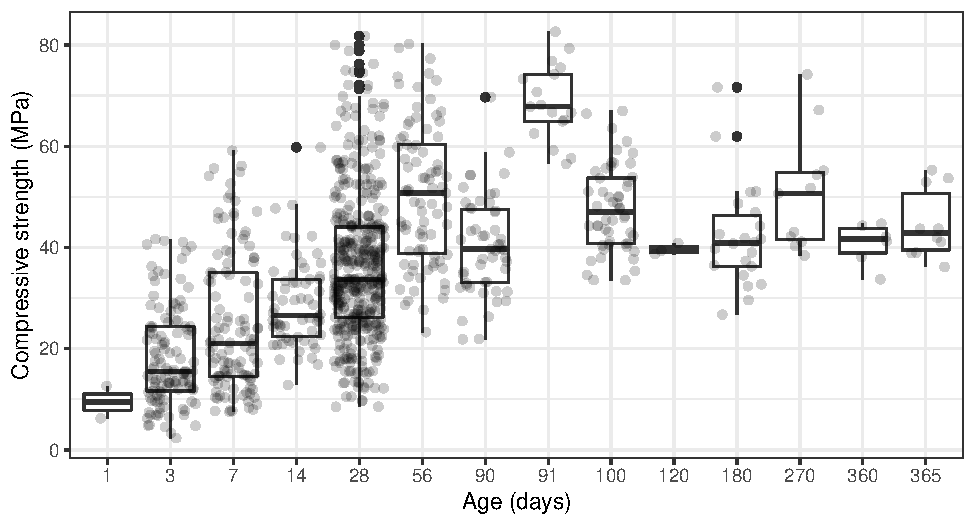
\includegraphics[scale=0.7]{Figures/boxplot.pdf}
\vspace{12pt}
\caption{Boxplot - compressive strength grouped by age}
\label{fig:boxplot}
\end{center}
\end{figure}
\vspace{8pt}

\begin{figure}[!ht]
\begin{center}
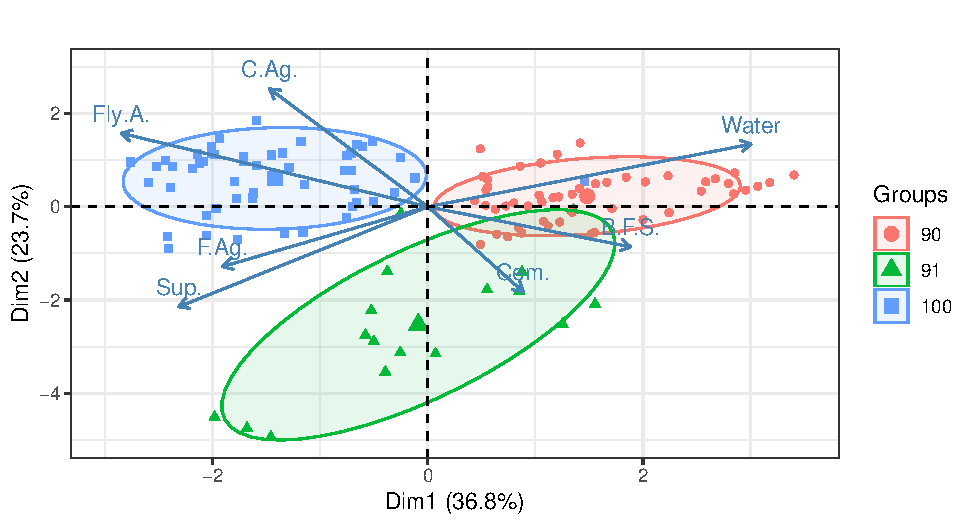
\includegraphics[scale=0.7]{Figures/pca-90-91-100.pdf}
\vspace{12pt}
\caption{Principal component analysis - 90, 91 and 100 days}
\label{fig:pca}
\end{center}
\end{figure}
\vspace{8pt}

After these manipulations, the final number of samples has been reduced from 1030 rows to 916 rows, with 416 different ingredient configurations (IDs). A xls file named "TODO" of the data at this point is available at the github repo (TODO: referencia).


% --------------------------------------------------------------------------
\subsection{Data visualization} \label{subsec:datavisualization}
% --------------------------------------------------------------------------

Several plots and tables were built to perform the exploration and visualization of the samples prepared in the previous step. Including analysis of the descriptive statistics of the continuous and categorical variables, the distribution of the variables in relation to the compressive strength, the correlation between the variables grouped by age, the relationship between the approximate mix and the compressive strength, the relationships between the main concrete ingredients and the compressive strength and principal component analysis (PCA) of the ingredients. All of these plots/tables are part of the extended version available on github. (TODO: reference). However, to keep the article short, here only the plots of the statistical analysis of the categorical variables are presented, in the Fig. \ref{fig:categorical}, which are used for an insight in the conclusion of this work.

\begin{figure}[!ht]
\begin{center}
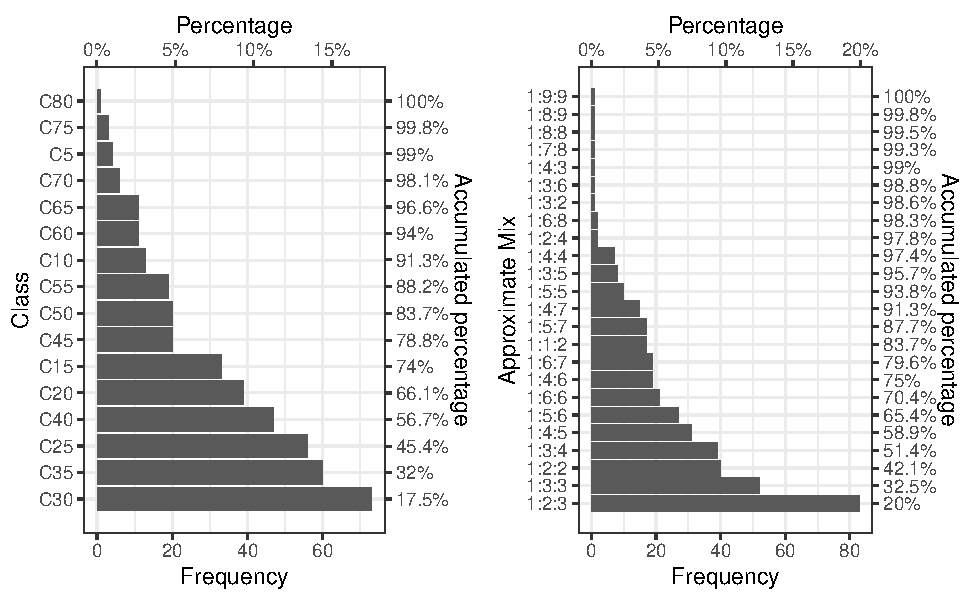
\includegraphics[scale=0.7]{Figures/stat-summ-categorical.pdf}
\vspace{12pt}
\caption{Descriptive statistics of the categorical variables}
\label{fig:categorical}
\end{center}
\end{figure}
\vspace{8pt}

% --------------------------------------------------------------------------
\subsection{Pre-processing and data split} \label{subsec:preprocessing}
% --------------------------------------------------------------------------

The main package used to build the machine learning models was the Caret Package \cite{caret}. It provides all functionalities and utilities to build prediction models for any data set, has a straight and clear documentation that guides the process and provide around 200 different algorithms to build models. In this work, it was done key steps described by \citet{irizarry2019} and \citet{Kuhn2008}. Starting by some pre-processing steps described below:


\begin{enumerate}

\item Removal of the categorical variables;

\item Separation of the dataset by age, resulting in 6 smaller datasets;

\item Removal of variables with near zero variance (only the fly ash of the 7-day set was removed);

\item Verification of variables with a correlation above 0.999, which did not occur;

\item Each data set was split into test and training sets, 20\% and 80\% respectively, shown in Table \ref{tab:split-config} and the distribution in the Fig. \ref{fig:split-dist}.

\end{enumerate}

\vspace{8pt}
\begin{table}[!ht]
\centering
\caption{Dataset split configurations}
\label{tab:split-config}
\vspace{6pt}
\begin{tabular}{cccc}
\hline
Model & Total samples & Train (80\%) & Test (20\%)\\ \hline
3 days & 121 & 97 & 24\\
7 days & 114 & 94 & 20\\
14 days & 62 & 50 & 12\\
28 days & 416 & 335 & 81\\
56 days & 83 & 67 & 16\\
100 days & 120 & 96 & 24\\ \hline
\end{tabular}
\end{table}
\vspace{8pt}

\begin{figure}[!ht]
\begin{center}
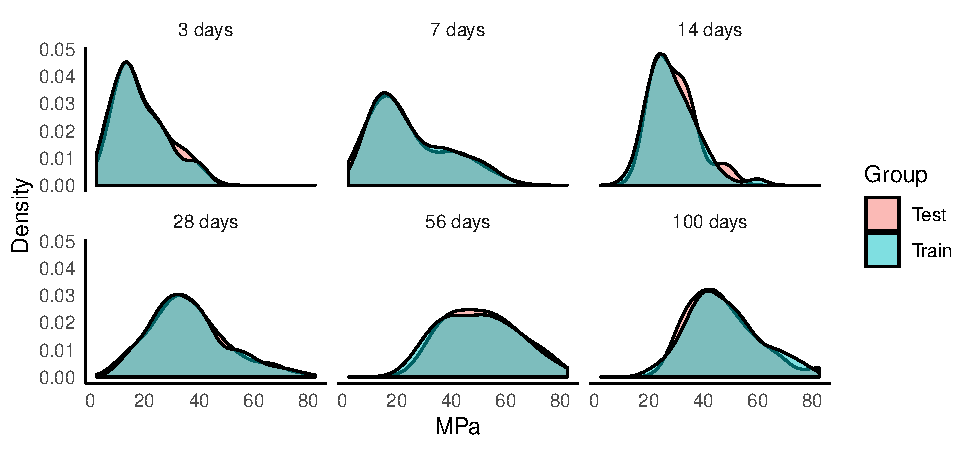
\includegraphics[scale=0.7]{Figures/dist-split.pdf}
\vspace{12pt}
\caption{Distribution of the test and train data in relation to compressive strength}
\label{fig:split-dist}
\end{center}
\end{figure}
\vspace{8pt}


% --------------------------------------------------------------------------
\subsection{Naive models} \label{subsec:naivemodels}
% --------------------------------------------------------------------------

Before building the real models, for comparison purposes, naive models were created. They simply predict that the compressive strength of the test set is the average compressive strength of the training set. In other words, naive models are simply the best guess possible to evaluate how close/far the real model is from a guess.


% --------------------------------------------------------------------------
\subsection{Machine learning models} \label{subsec:machinelearningmodels}
% --------------------------------------------------------------------------

We used only one algorithm in this work, chosen by the highest probability to achieve the best possible result, according to \citet{Fernandez2014}, who compared 179 algorithms across 121 different databases, and find out that the most likely to achieve the best possible results is the Parallel Random Forest (called prRF in the caret \cite{caret}). Six different models were built, one for each age-set, the following steps were made for each one:


\begin{enumerate}

\item Define the resampling scheme, with method of repeated cross validation;

\item Define a tuning grid for the "mtry" tuning parameter, which is a sequence from 1 to the number of columns of each dataset. All but the 7-day are equal since only the 7-day set have a column removed in the pre-processing;

\item Set seed equal to "1", chosen arbitrarily to guarantee reproducibility. This seed can be manipulated to obtain more satisfactory results, but it was chosen not to.

\item Do pre-processing transformation of the data with "center" and "scale" methods;

\item Run the caret "train" function with the above configurations and model "parRF";

\end{enumerate}


% --------------------------------------------------------------------------
\section{Results}\label{sec:Results}
% --------------------------------------------------------------------------
The performance evaluation of the models was performed by the Root Mean Square Error (RMSE). The RMSE is the measure used in all the works mentioned in the introduction allowing the comparison of the models in the discussion.

The test RMSE for each model in ascending order of age was 3.31, 4.36, 4.62, 4.72, 5.94 and 5.85 respectively. Table \ref{tab:results} presents the details and results of each model, including the naive one. Fig. \ref{fig:results} compares the actual and predicted values for the final models.

\vspace{8pt}
\begin{table}[!ht]
\centering
\caption{Final models results}
\label{tab:results}
\vspace{6pt}
\begin{tabular}{ccccccc}
\hline
Model & mtry & CV & Repetitions & Naive RMSE (test) & Final RMSE (train) & Final RMSE (test)\\ \hline
3 days & 6 & 30 & 10 & 9.303229 & 3.905196 & 3.310370\\
7 days & 2 & 10 & 10 & 13.443646 & 4.475981 & 4.361987\\
14 days & 13 & 30 & 10 & 7.593319 & 5.136687 & 4.620515\\
28 days & 11 & 30 & 10 & 14.283824 & 5.847334 & 4.716698\\
56 days & 8 & 30 & 10 & 12.702112 & 6.702565 & 5.939163\\
100 days & 8 & 10 & 10 & 12.614652 & 6.381940 & 5.851088\\ \hline
\end{tabular}
\end{table}
\vspace{8pt}

\begin{figure}[!ht]
\begin{center}
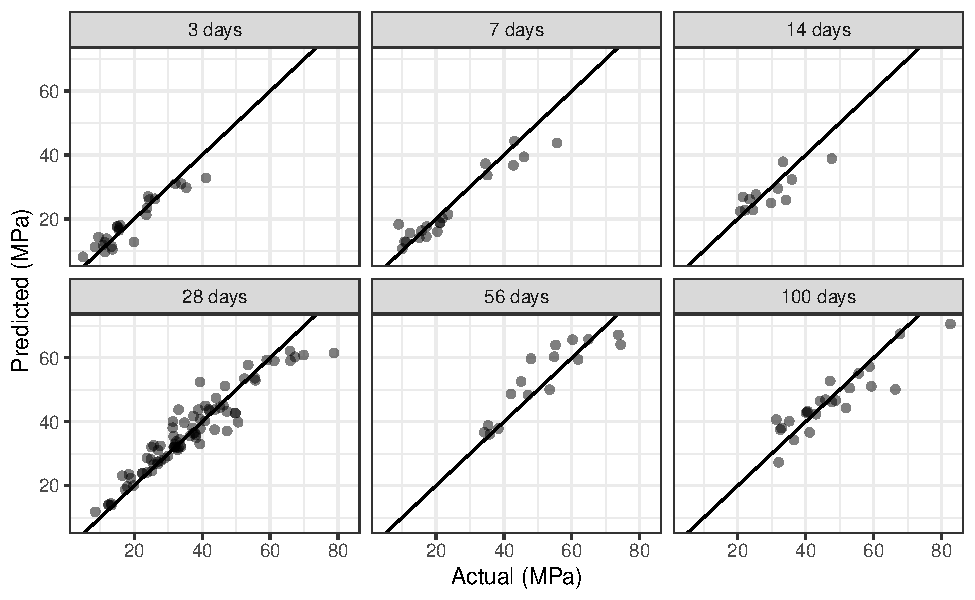
\includegraphics[scale=0.8]{Figures/results-comparison.pdf}
\vspace{12pt}
\caption{Actual vs predicted values for each model}
\label{fig:results}
\end{center}
\end{figure}
\vspace{8pt}

% --------------------------------------------------------------------------
\section{Discussion and conclusion}\label{sec:DiscussionAndConclusion}
% --------------------------------------------------------------------------

The models built present satisfactory results and prove that the compressive strength of concrete can be predicted relatively easily.The alternative adopted, to create a model for each set of age proved to be a valid method, instead of using the age as a predictor along with the ingredients like the related studies with the same dataset. The adoption of this stratification achieved different results for each age group. However, the RMSE calculated in our work and the one obtained in the related works were close. Table \ref{tab:comparison} shows the comparison between these studies and the 28 days model developed here.

\vspace{8pt}
\begin{table}[!ht]
\centering
\caption{Comparison to other works with same dataset}
\label{tab:comparison}
\vspace{6pt}
\begin{tabular}{lclcc}
\hline
Author & Year & Algorithm & RMSE & Difference ({\%}) \\ \hline
\citet{Pierobon2018} & 2018 & 5 algorithms Ensemble & 4.150 & -12\\
\textbf{This work (28 day)} & \textbf{2020} & \textbf{Parallel Random Forest} & \textbf{4.717}  & \textbf{0}\\
\citet{Hameed2020} & 2020 & Artificial Neural Networks & 4.736 & 0\\
\citet{Raj2018} & 2018 & Gradient Boosting Regressor & 4.957  & +5\\
\citet{Modukuru2020} & 2020 & Random Forest Regressor & 5.080  & +8\\
\citet{Alshamiri2020} & 2020 & Regularized Extreme Learning Machine & 5.508 & +17\\
\citet{Abban2016} & 2016 & SVM with Radial Basis Function Kernel & 6.105 & +29\\ \hline
\end{tabular}
\end{table}
\vspace{8pt}


Following the line of reasoning of this work, the same hypothesis can be evaluated using other algorithms besides the one used here (Parallel Random Forest), as they can present better results. Another option is to create an ensemble of various algorithms, just like \citet{Pierobon2018}, but with the separation of age sets proposed here. In addition, this study can be reproduced with a larger dataset, ideally with a similar number of samples in each age group and a more homogeneous distribution of compressive strength.


%--------------------------------------------------------------------------
\vspace{20pt}
\noindent \textbf{Authorship statement.} The authors hereby confirm that they are the sole liable persons responsible for the authorship of this work, and that all material that has been herein included as part of the present paper is either the property (and authorship) of the authors, or has the permission of the owners to be included here. 

\bibliography{bibliography}

\end{document}
% --------------------------------------------------------------------------